%%
%% Author: papian
%% 26/05/18
%%



\documentclass{bredelebeamer}




%%%%%%%%%%%%%%%%%%%%%%%%%%%%%%%%%%%%%%%%%%%%%%%%



\title[OS Project]{Operating System Project}
% Titre du diaporama

\subtitle{An implementation of server-client database using non-blocking operations}
% Sous-titre optionnel

\author{Julmy, S., Papinutto, M. \& Veillard, S.}
% La commande \inst{...} Permet d'afficher l' affiliation de l'intervenant.
% Si il y a plusieurs intervenants: Marcel Dupont\inst{1}, Roger Durand\inst{2}
% Il suffit alors d'ajouter un autre institut sur le modèle ci-dessous.

\institute[UniFr]{}


\date{30 Septembre 2018}
% Optionnel. La date, généralement celle du jour de la conférence

\subject{Presentation projet OS Group 4 Sylvain Julmy, Michael Papinutto et Sami Veillard}
% C'est utilisé dans les métadonnes du PDF

\logo{
\includegraphics[scale=0.5]{../report/images/unifrlogo.jpg}}

%%%%%%%%%%%%%%%%%%%%%%%%%%%%%%%%%%%%%%%%%%%%%%%%%%%%%%%%%%%%%%%%%%%%%
\begin{document}

    \begin{frame}
        \titlepage
    \end{frame}


    \section{Selected Approach}

    \begin{frame}{Multithreaded Server}
        We selected a multi-threaded server as: \\
        \begin{itemize}
            \item Allows to access same data structure
            \item light weight as compared to multi-process server
            \item easier to implement
        \end{itemize}
    \end{frame}

     \begin{frame}{To use Mutex or not to use Mutex}

         Our lock-free implementation allowed us not to use Mutex \\

        \begin{itemize}
            \item No need to prioritize read or write operations
            \item No dreadlock problems
            \item All clients have the same right to access the data structure at any time
        \end{itemize}
    \end{frame}

     \begin{frame}{non-blocking operations}

        Non-blocking operations use atomic operations allowing to perform several action at each clock cycle\\
        As the actions are perform in one cycle it is not crucial to wait for the operation to be completed \\
        In c atomic operations functionnality such as CompareAndSet can be done by "stealing" a bit from a pointer
        using bit-wise operators to extract the pointer and the mark from a single word \\

        \begin{itemize}
            \item Swap values exemple
        \end{itemize}
    \end{frame}

     \begin{frame}{Reversed Split-Ordered Hash-Set}
        This implementation offers a rapid access to the data but might require slightly more memory that other data-structure
        \begin{itemize}
            \item Buckets are linked to a stack as the list grows supplemental buckets references are added so that buckets is keep small
            \item Require to set up sentinel bucket in order to avoid "corner case" that occurs when deleting a reference by a bucket reference
            \item The sentinel bucket is never deleted
        \end{itemize}
         \begin{figure}
             \centering
             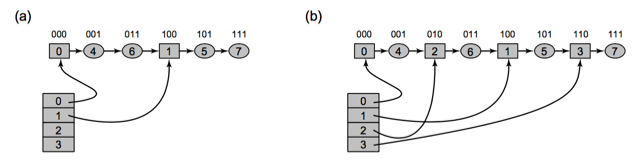
\includegraphics{hashsetFig1}
         \end{figure}
    \end{frame}

     \begin{frame}{Operation add in this Hash-Set}
         Scheme of the procedure that add the key 10 to the lock-free hash-set
         \begin{figure}
             \centering
             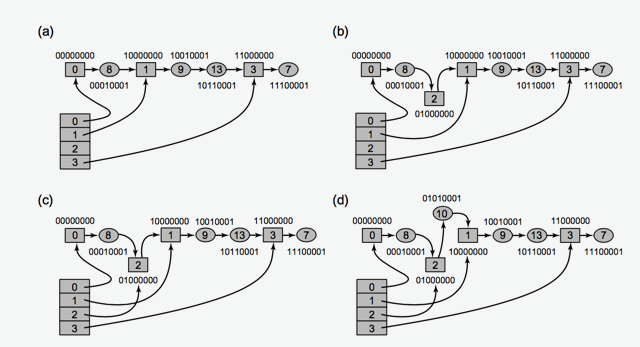
\includegraphics{hashsetFig2}
         \end{figure}
    \end{frame}

    \setion{Test}

    \begin{frame}{Multithreaded Server}
        Texte normal \alert{Texte Alert}  \exemple{Texte exemple} \emph{Texte emphase}

        \begin{columns}

            \begin{column}{0.5\textwidth}
                \begin{block}{Bloc simple}
                    \begin{itemize}
                        \item Premier point
                    \end{itemize}
                \end{block}

                \begin{exampleblock}{Bloc exemple}
                    \begin{itemize}
                        \item Premier point
                    \end{itemize}
                \end{exampleblock}

                \begin{alertblock}{Bloc alert}
                    \begin{itemize}
                        \item Premier point
                    \end{itemize}
                \end{alertblock}

            \end{column}

            \begin{column}{0.5\textwidth}
                \boiteviolette{
                Une boite violette
                }

                \boiteorange{
                Une boite orange
                }

                \boitegrise{
                Une boite grise
                }



                \begin{tcolorbox}[tabvert,tabularx={X||Y|Y|Y|Y||Y}, boxrule=0.5pt, title=Mon tableau des prix]
                    Couleur & Prix 1  & Prix 2  & Prix 3 \\\hline\hline
                    Rouge   & 10.00   & 20.00   &  30.00 \\\hline
                    Vert    & 20.00   & 30.00   &  40.00  \\\hline
                    Bleu    & 30.00   & 40.00   &  50.00 \\\hline\hline
                    Orange  & 60.00   & 90.00   & 120.00
                \end{tcolorbox}

            \end{column}

        \end{columns}
    \end{frame}




    \section{Les blocs}

    \begin{frame}{Les blocs}

        \begin{block}{Bloc simple}
            \begin{itemize}
                \item Premier point
                \item Second point
                \item Troisième point
            \end{itemize}
        \end{block}

        \begin{exampleblock}{Bloc exemple}
            \begin{itemize}
                \item Premier point
                \item Second point
                \item Troisième point
            \end{itemize}
        \end{exampleblock}

        \begin{alertblock}{Bloc alert}
            \begin{itemize}
                \item Premier point
                \item Second point
                \item Troisième point
            \end{itemize}
        \end{alertblock}
    \end{frame}


    \section{Les bo\^ites}

    \begin{frame}{Les boites}

        \begin{columns}

            \begin{column}{0.5\textwidth}
                \boitejaune{
                Ceci est \\
                une boite jaune
                }

                \boiteorange{
                Ceci est \\
                une boite orange
                }

                \boitemarron{
                Ceci est \\
                une boite marron
                }
            \end{column}

            \begin{column}{0.5\textwidth}
                \boiteviolette{
                Ceci est \\
                une boite violette
                }

                \boitebleue{
                Ceci est \\
                une boite bleue
                }

                \boitegrise{
                Ceci est \\
                une boite grise
                }

            \end{column}

        \end{columns}


    \end{frame}



    \section{Les listes}
    \subsection{Liste à item}

    \begin{frame}{Titre de la frame}

        \begin{itemize}
            \item premier élément de liste,
            \item deuxième élément de liste,
            \item troisième élément de liste.
        \end{itemize}
    \end{frame}

    \subsection{Liste énumérative}
    \begin{frame}{Titre de la frame}
        \begin{enumerate}
            \item élément de liste numéro 1,
            \item élément de liste numéro 2,
            \item élément de liste numéro 3.
        \end{enumerate}
    \end{frame}


    \subsection{Liste descriptive}
    \begin{frame}{Titre de la frame}
        \begin{description}
            \item [Thème de présentation : ] ces thèmes sont en fait...
            \item [Thème de couleur : ] gère tout ce qui est couleur...
            \item [Thème de police : ] s'occupe de tout ce qui est police, gras...
            \item [Thème interne : ] s'occupe de l'apparence des éléments...
        \end{description}
    \end{frame}



    \section{Le texte}

    \begin{frame}{Titre de la frame}

        Voici du texte normal

        \alert{Voici du texte \texttt{alert}}

        \exemple{Voici du texte \texttt{exemple}}

        \emph{Voici du texte \texttt{emphase}}

    \end{frame}


    \section{Les tableaux}

    \begin{frame}{Tableaux}

        % merci: http://tex.stackexchange.com/questions/112343/beautiful-table-samples

        \begin{tcolorbox}[tabjaune,tabularx={X||Y|Y|Y|Y||Y}, boxrule=0.5pt]
            Couleur & Prix 1  & Prix 2  & Prix 3   & Prix 4   & Prix 5 \\\hline\hline
            Rouge   & 10.00   & 20.00   &  30.00   &  40.00   & 100.00 \\\hline
            Vert    & 20.00   & 30.00   &  40.00   &  50.00   & 140.00 \\\hline
            Bleu    & 30.00   & 40.00   &  50.00   &  60.00   & 180.00 \\\hline\hline
            Orange  & 60.00   & 90.00   & 120.00   & 150.00   & 420.00
        \end{tcolorbox}

        \begin{tcolorbox}[tabvert,tabularx={X||Y|Y|Y|Y||Y}, boxrule=0.5pt, title=Mon tableau des prix]
            Couleur & Prix 1  & Prix 2  & Prix 3   & Prix 4   & Prix 5 \\\hline\hline
            Rouge   & 10.00   & 20.00   &  30.00   &  40.00   & 100.00 \\\hline
            Vert    & 20.00   & 30.00   &  40.00   &  50.00   & 140.00 \\\hline
            Bleu    & 30.00   & 40.00   &  50.00   &  60.00   & 180.00 \\\hline\hline
            Orange  & 60.00   & 90.00   & 120.00   & 150.00   & 420.00
        \end{tcolorbox}

    \end{frame}


    \begin{frame}{Tableaux}

        % merci: http://tex.stackexchange.com/questions/112343/beautiful-table-samples

        \begin{tcolorbox}[tabgris,tabularx={X||Y|Y|Y|Y||Y}, boxrule=0.5pt]
            Couleur & Prix 1  & Prix 2  & Prix 3   & Prix 4   & Prix 5 \\\hline\hline
            Rouge   & 10.00   & 20.00   &  30.00   &  40.00   & 100.00 \\\hline
            Vert    & 20.00   & 30.00   &  40.00   &  50.00   & 140.00 \\\hline
            Bleu    & 30.00   & 40.00   &  50.00   &  60.00   & 180.00 \\\hline\hline
            Orange  & 60.00   & 90.00   & 120.00   & 150.00   & 420.00
        \end{tcolorbox}

        \begin{tcolorbox}[taborange,tabularx={X||Y|Y|Y|Y||Y}, boxrule=0.5pt, title=Mon tableau des prix]
            Couleur & Prix 1  & Prix 2  & Prix 3   & Prix 4   & Prix 5 \\\hline\hline
            Rouge   & 10.00   & 20.00   &  30.00   &  40.00   & 100.00 \\\hline
            Vert    & 20.00   & 30.00   &  40.00   &  50.00   & 140.00 \\\hline
            Bleu    & 30.00   & 40.00   &  50.00   &  60.00   & 180.00 \\\hline\hline
            Orange  & 60.00   & 90.00   & 120.00   & 150.00   & 420.00
        \end{tcolorbox}

    \end{frame}



    \section{Les images}

    \begin{frame}{Titre de la frame}

        \begin{figure}
            \centering
            \includegraphics[scale=0.5]{images/architecturebretonne_wikipedia.jpg}
            \caption{Éléments d'architecture bretonne typique du Sud de la France. (\href{http://commons.wikimedia.org/wiki/File:Colmar_-_Alsace.jpg}{Wikipédia.fr} CC-By-Sa)}
        \end{figure}

    \end{frame}



\end{document}
